\documentclass[a4paper,11pt]{article}
\title{PAG: Determination of the half-thickness of aluminium}
\author{Izaak van Dongen}

% make the document take up more of the page
\usepackage[margin=1in,headheight=13.6pt]{geometry}

% so the title can be accessed by fancyhdr (and is automatically correctly
% spelled etc)
\makeatletter
\let\thetitle\@title
\makeatother

% custom document header/footer
\usepackage{fancyhdr}
\usepackage{lastpage}

\pagestyle{fancy}
\fancyhf{}
\lhead{\thetitle}
\rhead{Izaak van Dongen}
\rfoot{Page \thepage\ of \pageref{LastPage}}

%% fonts
%\usepackage[p,osf]{cochineal}
%\usepackage[scale=.95,type1]{cabin}
%\usepackage[cochineal,bigdelims,cmintegrals,vvarbb]{newtxmath}
%% fixed width font with 80 chars per listing line
%\usepackage[scaled=.94]{newtxtt}
%\usepackage[cal=boondoxo]{mathalfa}
\usepackage{amsfonts}

% provides eg uptau
\usepackage{upgreek}

% maths symbols and other stuff (supersedes the ams* packages)
\usepackage{mathtools}

% for typesetting differentials
\usepackage{commath}

%
\usepackage{yfonts}
\def\initdefault{yinit} % fix weird font thing

% define starting paragraph letter stuff
\usepackage{lettrine}
\setcounter{DefaultLines}{4}
\setlength{\DefaultFindent}{0.5em}
\setlength{\DefaultNindent}{0em}
\renewcommand{\LettrineFontHook}{\usefont{U}{yinit}{m}{n}}


% no paragraph indent
\usepackage[parfill]{parskip}

% pretty table rules and multirow entries. Also page-breaking tables
\usepackage{booktabs}
\usepackage{multirow}
\usepackage{longtable}

% plotting mathematical functions (needs version request)
\usepackage{pgfplots}
\pgfplotsset{compat=1.15}

% \url function and clickable table of contents. no ugly red boxes though
\usepackage[hidelinks]{hyperref}

% For framing definitions
\usepackage[framemethod=tikz]{mdframed}
\usepackage[most]{tcolorbox}

\newtcolorbox{definition}{
freelance,
before=\par\vspace{2\bigskipamount}\noindent,
after=\par\bigskip,
frame code={
  \node[
  anchor=south west,
  inner xsep=8pt,
  xshift=8pt,
  rounded corners=5pt,
  font=\bfseries\color{white},
  fill=gray] at (frame.north west) (tit) {\strut Definition:};
  \draw[
  line width=3pt,
  rounded corners=5pt,gray
  ] (tit.west) -| (frame.south west) -- ([xshift=15pt]frame.south west);
},
interior code={},
top=2pt
}

% for better table of contents stuff, providing the \listof* commands and not
% listing the tables in the table of contents
\usepackage[nottoc,notlof,notlot]{tocbibind}

% more advanced handling of utf8 and fonts or something. apparently good to have
\usepackage[utf8]{inputenc}
\usepackage[T1]{fontenc}

% somehow this fixes ~ signs in listing environments
\usepackage{lmodern}

% bibliography management with square braces for citations
\usepackage[square,numbers]{natbib}

% graphics, like eps files and stuff (supersedes graphics)
\usepackage{graphicx}

% used to horizontally align floats
\usepackage{subfig}

% used for figures
\usepackage{float}

% needed for colouring and stuff (xcolor supersedes color)
\usepackage{xcolor}

\definecolor{codegreen}{rgb}{ 0,0.6,0}

% listings of code
\usepackage{minted}
\setminted{breaklines,
           breakbytokenanywhere,
           linenos
}
\usemintedstyle{friendly}
% bigger line numbers
\renewcommand\theFancyVerbLine{\footnotesize\arabic{FancyVerbLine}}

% that can break across pages while being captioned figures
\usepackage{caption}
\newenvironment{longlisting}
{\addvspace{\baselineskip}\captionsetup{type=listing}}
{\addvspace{\baselineskip}}

% allow maths to break across pages
\allowdisplaybreaks

\usepackage[separate-uncertainty]{siunitx}

\begin{document}
    \maketitle%\thispagestyle{empty} % no page number under title

    \lettrine{B}{y linear regression} of \(\ln(I/\si{\becquerel})\) (Figure
    \ref{fig_log_plot}) against \(x/\si{\milli\metre}\), I determined the value
    of the half thickness of aluminium as \(x_{1/2} = \SI{0.0003796}{\metre}\),
    or about \(\SI{0.38}{\milli\metre}\). As an order of magnitude, this is
    consistent with common sense, as, very roughly speaking, the intensity
    halved when adding about \(\SI{0.5}{\milli\metre}\) of aluminium.

    A less precise calculation from the fitted exponential curve in Figure
    \ref{fig_exp_plot}, and particularly the consideration of the points
    \((\SI{0.515}{\milli\metre}, \SI{18.00}{\becquerel})\) and
    \((\SI{0.894}{\milli\metre}, \SI{9.01}{\becquerel})\) suggests a
    half-thickness of about \((0.894 - 0.515)\si{\milli\metre} =
    \SI{0.379}{\milli\metre}\), which is consistent with the actual analysis.

\begin{longlisting}
\inputminted{R}{analyse.r}
\caption{Source code of the program \texttt{analyse.r}.}
\label{lst_analyse}
\end{longlisting}

\begin{longlisting}
\inputminted{text}{analysis_output.txt}
\caption{Output of \texttt{analyse.r} (\ref{lst_analyse}) when run.}
\label{lst_results}
\end{longlisting}

\begin{figure}[H]
\begin{center}
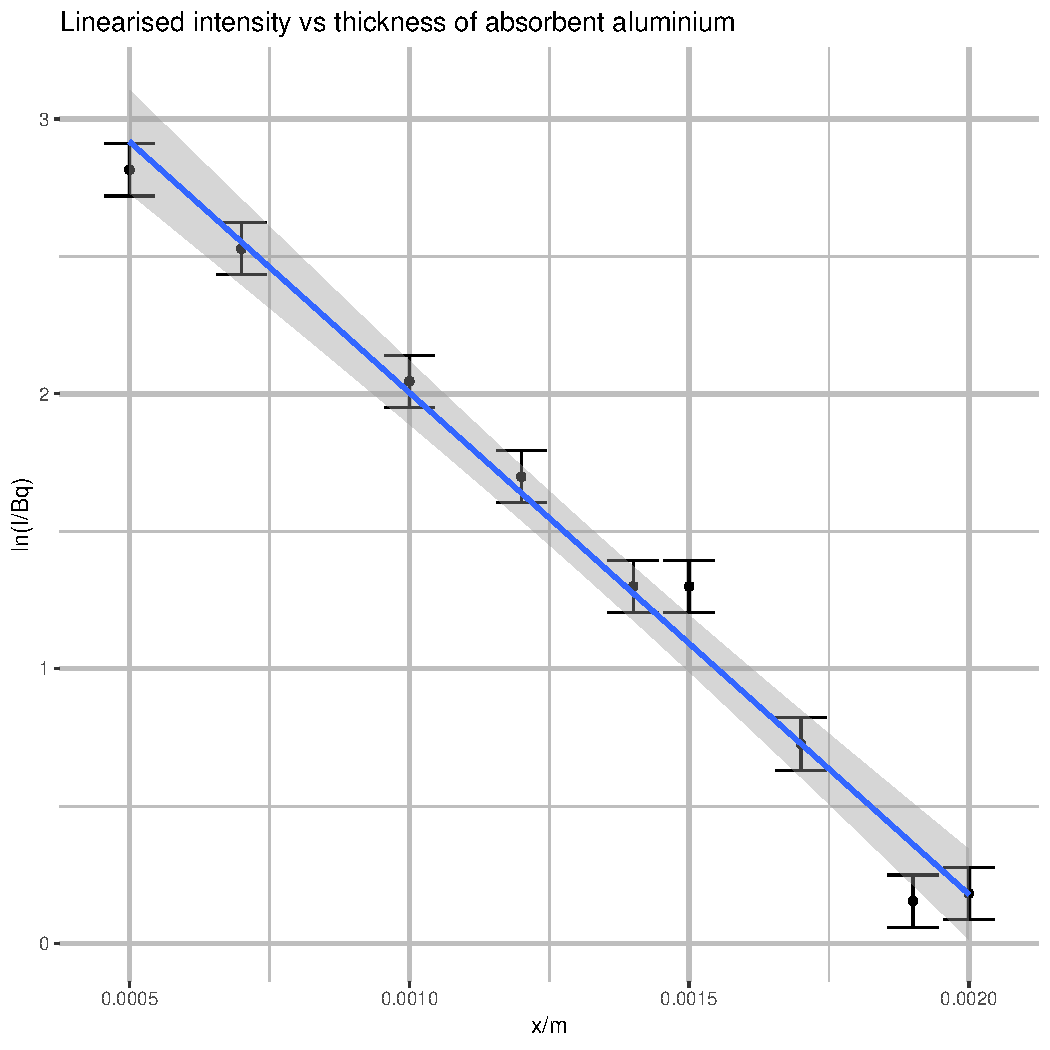
\includegraphics[width=0.9\textwidth,page=1]{Rplots.pdf}
\end{center}
\caption{Plot of \(\ln(I/\si{\becquerel})\) against \(x / \si{\milli\metre}\)}
\label{fig_log_plot}
\end{figure}

\begin{figure}[H]
\begin{center}
\includegraphics[width=0.9\textwidth,page=2]{Rplots.pdf}
\end{center}
\caption{Plot of maximum displacements in experiment 2.}
\label{fig_exp_plot}
\end{figure}


\end{document}
